\documentclass{beamer}
\usepackage{graphicx}
\title{Academic Writing 101}
\author{Dr.~Junchen~Feng}
\date{January 2025}

\begin{document}

\maketitle

\begin{frame}
    \begin{itemize}
        \item Structure
        \item Style
        \item How to Use LLM Creatively and Responsibly
    \end{itemize}
\end{frame}


\begin{frame}
\frametitle{1 Structure}
\begin{itemize}
    \item Title
    \item Abstract
    \item Introduction (Literature Review)
    \item Methodology
    \item Results/Analysis
    \item Discussion
\end{itemize}
\end{frame}
    

\begin{frame}
    \frametitle{1.1 Introduction}
    \begin{itemize}
        \item \textbf{Why the reader should care about your research}
        \begin{itemize}
            \item introduce your research question,
            \item identify why the question needs to be asked 
            \item state the hypothesis you are testing.
        \end{itemize}
    \end{itemize}
    \end{frame}
    
    \begin{frame}
    \frametitle{1.1 What is a research question?}    
    \begin{itemize}
    
    \item \textbf{Good, bad, ugly}:
    \begin{itemize}
        \item This paper is about handwriting recognition
        \item This paper uses CNN to recognize handwriting
        \item This paper studies if dropout improves handwriting recognition with Lenet-5
    \end{itemize}
    
    \item \textbf{Great}:
    
    \begin{quote}
        This paper studies if randomly masking certain coefficients during training (dropout) can prevent Lenet-5 from overfitting, and thus improves handwriting recognition task performance on MNIST dataset.
    \end{quote}
    
    \end{itemize}
    \end{frame}
    
    
    
    \begin{frame}
    \frametitle{1.2 Literature Review}
    \begin{itemize}
        \item \textbf{The Reverse Triangle}
        \item \textbf{Steps}:
        \begin{itemize}
            \item Survey the field to understand the broader context.
            \item Identify key debates and research gaps.
            \item How your research contributes to the field by closing the gap
        \end{itemize}
    \end{itemize}
    \end{frame}
    
    \begin{frame}
    \frametitle{Example}
    \begin{itemize}
        \item Handwriting recognition is a longstanding problem in the field of computer vision ...
        \item The Lenet-5 model (LeCun et al., 1998) significantly improved the performances by using CNN to automatically learning features from raw images.
        \item However, research (So and so, 200x; So and so,200y) shows that CNN is prone to overfitting. Recently Hinton et al. (2014) proposed a new method called dropout that randomly masks certain coefficients during training.
        \item This paper attempts to apply dropout to improve the performance of Lenet-5 model in handwriting recognition
    \end{itemize}
    \end{frame}
    
    
    
    \begin{frame}
    \frametitle{1.3 Methodology: Reproduces My Research for Dummies}
    \begin{itemize}
        \item \textbf{Data Source}: Specify how the data were collected and what is in the dataset.
        \item \textbf{Analysis Protocal}: Detail the research design and every research step
    \end{itemize}
    \end{frame}
    
    
    \begin{frame}
        \frametitle{Example A}
        \begin{itemize}
            \item The Experiment design is compare lenet-5 and lenet-5 with dropout on MNIST dataset.
            \item The MNIST dataset is ...  The dataset is from ... . Here a few example...
            \item The lenet-5 model is specified as ... . The dropout is specified as ... .
            \item The both models are trained with ... optimizer, ... loss function, ... config
        \end{itemize}
        \end{frame}
        
        
    \begin{frame}
    \frametitle{Example B}
    \begin{itemize}
        \item This paper tests GAD-7 and LLM-Diagnosis system on 15 volunteers to compare their accuracy and patient experience.
        \item The volunteers are recruited from ... . The volunteers have x men and y women, aging from a to b ...
        \item The GAD-7 is ..., administered by ... 
        \item The LLM Diagnosis system is ... . Its key prompt is ... . Its user interface is ... . Here is a screenshot and an excerpt of user conversation.
    \end{itemize}
    \end{frame}
    
    
    
    \begin{frame}
    \frametitle{1.4 Results/Analysis}
    \begin{itemize}
        \item \textbf{Describe the results literally and "figuratively"}
        \begin{itemize}
            \item You need to describe the tables and graphs in WORDS.
            \item Callback to your methodology if necessary.
        \end{itemize}
        \item \textbf{Highlight Your Insight}:
        \begin{itemize}
            \item Except for the summary statistics, you need to explicitly state the key findings for each table and graph.
            \item Ideally each paragraph builds or leads to your final Aha moment.
        \end{itemize}
    \end{itemize}
    \end{frame}
    
    \begin{frame}
    \frametitle{Dos and Don'ts for Tables and Graphs}
    \begin{itemize}
        \item Prefer tables over graphs. Prefer simplicity over complexity.
        \item Retain only the most important information. The rest goes to the appendix.
        \item Pay attention to X axis, Y axis, Legend
        \item Avoid using colors in graphs.
    \end{itemize}
    \end{frame}
    
    \begin{frame}
        \frametitle{Graph as a Story Teller}
        \begin{minipage}{0.48\textwidth}
            \begin{figure}
                \centering
                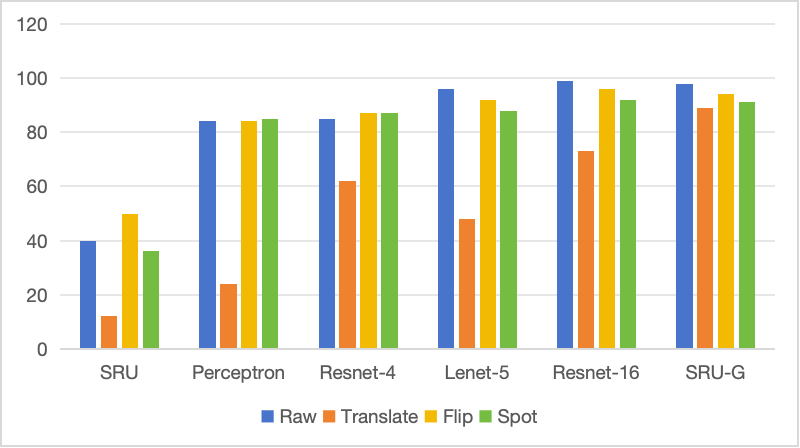
\includegraphics[width=\textwidth]{fig-1.png}
            \end{figure}
        \end{minipage}
        \hfill
        \begin{minipage}{0.48\textwidth}
            \begin{figure}
                \centering
                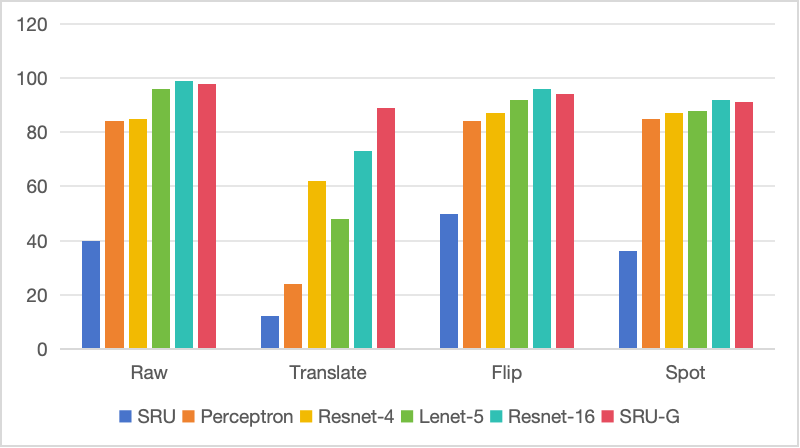
\includegraphics[width=\textwidth]{fig-2.png}
            \end{figure}
        \end{minipage}
    \end{frame}
    
    \begin{frame}
        \frametitle{Graph as a Story Teller}
        \begin{minipage}{0.48\textwidth}
            \begin{figure}
                \centering
                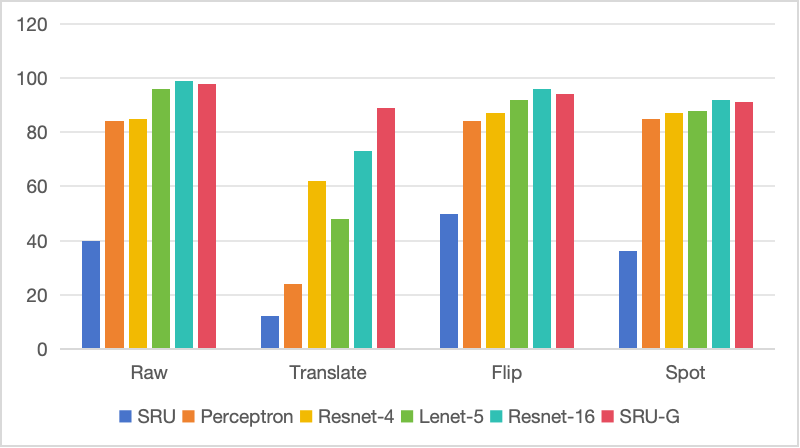
\includegraphics[width=\textwidth]{fig-2.png}
            \end{figure}
        \end{minipage}
        \hfill
        \begin{minipage}{0.48\textwidth}
            \begin{figure}
                \centering
                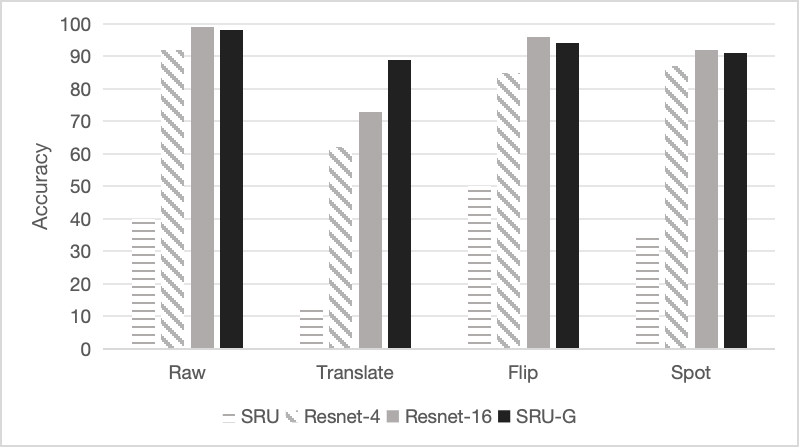
\includegraphics[width=\textwidth]{fig-3.png}
            \end{figure}
        \end{minipage}
    \end{frame}
    
    \begin{frame}
        \frametitle{Prefer Table over Graph}
        \begin{minipage}{0.48\textwidth}
            \begin{figure}
                \centering
                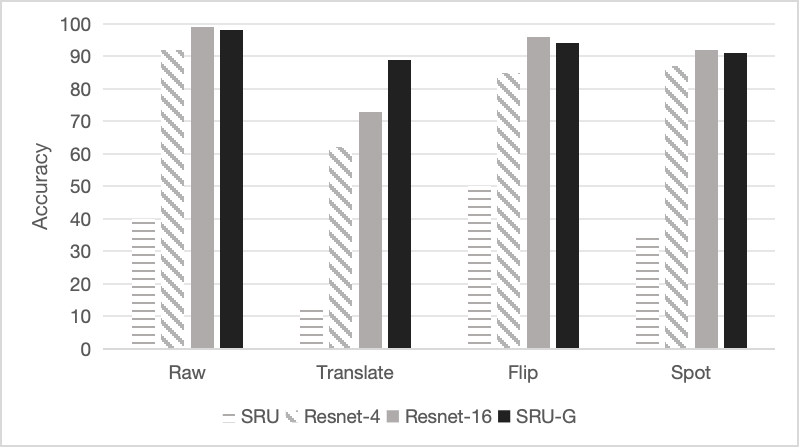
\includegraphics[width=\textwidth]{fig-3.png}
            \end{figure}
        \end{minipage}
        \hfill
        \begin{minipage}{0.48\textwidth}
    
            \begin{table}[h]
                \centering
                \resizebox{0.8\textwidth}{!}{%
                \begin{tabular}{|l|c|c|c|c|}
                    \hline
                    & SRU & Resnet-4 & Resnet-16 & SRU-G \\
                    \hline
                    Raw & 40 & 92 & \textbf{99} & 98 \\
                    \hline
                    Translate & 12 & 62 & 73 & \textbf{89} \\
                    \hline
                    Flip & 50 & 85 & \textbf{96} & 94 \\
                    \hline
                    Spot & 36 & 87 & \textbf{92} & 91 \\
                    \hline
                \end{tabular}
                }
            \end{table}
            \end{minipage}
    
    \end{frame}
    
    
    \begin{frame}
    \frametitle{How to Interpret}
    \begin{itemize}
        \item SRU-G is translate-invariant while has comparable performance to the SOTA model other scenarios
        \item Graph X demonstrates that the SRU-G is translate-invariant while has comparable performance to the Resnet-16(SOTA) in other scenarios.
        The SRU-G achieves 89\% accuracy on the translate dataset, outperforming the SOTA Resnet-16 by 16\%, while trailing the SOTA model in other scenarios by a narrow margin of 1.5\% on average.
        The SRU-G outperforms the baseline models that motivates the research. The baseline SRU model is the weakest model in the raw dataset and is suspectible to noise, especially the translation noise. The Resnet-4 has similar depth as the SRU-G but its accuracy is on average 15\% lower than the SRU-G.
        The experiment data show that the shallow SRU-G is robust to translation and has a competitive overall performance to the SOTA model.
    \end{itemize}
    \end{frame}
    
    
    \begin{frame}
    \frametitle{1.5 Discussion}
    \begin{itemize}
        \item \textbf{What Have You Found}: Summarize your main findings and connect them to the existing body of research.
        \item \textbf{How it Helps the Community}: Discuss how your results help the community connect the dots and fill gaps.
        \item \textbf{What the Community Can Do Next}: Suggest areas for future research or practical applications based on your findings.
    \end{itemize}
    \end{frame}
    
    \begin{frame}
    \frametitle{1.6 Abstract: Short But to the Point}
    \begin{itemize}
        \item State the main objectives of the study.
        \item Describe the methods used.
        \item Summarize key results and conclusions.
    \end{itemize}
    \end{frame}
    
    \begin{frame}
    \frametitle{1.7 Title}
    \begin{itemize}
        \item \textbf{Model Paper}: A clear description the problem it solved
        \item "Dropout: A Simple Way to Prevent Neural Networks from Overfitting"
        \item \textbf{Application Paper}:A dramatic reveal of the research punchline
        \item "Dancing With Glass Manacles: How Negative Stereotypes Affect Highly-Educated Women in the Chinese Marriage Market"
    \end{itemize}
    \end{frame}
    
    \begin{frame}
    \frametitle{2 Literary Writing V.S. Academic Writing}
    \begin{quote}
        The (2nd) challenge of academic writing is to convey your complex thinking process to the reader with minimum information loss when the reader cannot engage in dialogue.
    \end{quote}
    \begin{itemize}
        \item Write for the reader's thinking process
        \item It's good to repeat yourself
    \end{itemize}
    \end{frame}
    
    \begin{frame}
        \frametitle{2.2 Understanding by Design}
        \begin{itemize}
            \item Like prompting, you need to make your implicit context explicit to the reader
            \item You can use jargon and acronyms. For general audiences, explain them first. For field experts, use them directly.
            \item Anticipate your reader's questions and answer them "preemptively" in the text
        \end{itemize}
    \end{frame}
    
    \begin{frame}
    \frametitle{2.2 An example}
    Graph X demonstrates that the SRU-G is translate-invariant while has comparable performance to the \textbf{Resnet-16(SOTA)} in other scenarios.
    The SRU-G achieves 89\% accuracy on the translate dataset, outperforming \textbf{the SOTA Resnet-16} by 16\%, while trailing \textbf{the SOTA model} in other scenarios by a narrow margin of 1.5\% on average.
    SRU-G outperforms the baseline models that motivates the research. The baseline SRU model is the weakest model in the raw dataset and is suspectible to noise, especially the translation noise. \textbf{The Resnet-4 has similar depth as the SRU-G but its accuracy is on average 15\% lower than the SRU-G.}
    The experiment data show that the shallow SRU-G is robust to translation and has a competitive overall performance to \textbf{the SOTA model}.
    \end{frame}
    
    
    \begin{frame}
        \frametitle{2.3 Repetition is Good}
        \begin{itemize}
            \item The easiest way to make audience remember is to repeat it again and again, even unconsciously.
            \item Intentional reptition leaves a trail for your reader to follow.
            \item Repeat ideas, not expressions.
        \end{itemize}
    \end{frame}
    
    \begin{frame}
        \frametitle{2.2 Revisit the Interpretation}
        Graph X demonstrates that the \textbf{SRU-G} is translate-invariant while has comparable performance to the Resnet-16(SOTA) in other scenarios.
        The \textbf{SRU-G} achieves 89\% accuracy on the translate dataset, outperforming the SOTA Resnet-16 by 16\%, while trailing the SOTA model in other scenarios by a narrow margin of 1.5\% on average.
        \textbf{SRU-G} outperforms the baseline models that motivates the research. The baseline SRU model is the weakest model in the raw dataset and is suspectible to noise, especially the translation noise. The Resnet-4 has similar depth as the SRU-G but its accuracy is on average 15\% lower than the \textbf{SRU-G}.
        The experiment data show that the shallow \textbf{SRU-G} is robust to translation and has a competitive overall performance to the SOTA model.
        \end{frame}
    
    
    \begin{frame}
        \frametitle{2.2 Revisit the Interpretation Again}
        Graph X demonstrates that the SRU-G is \textbf{translate-invariant} while has comparable performance to the Resnet-16(SOTA) in other scenarios.
        The SRU-G achieves 89\% accuracy on \textbf{the translate dataset}, outperforming the SOTA Resnet-16 by 16\%, while trailing the SOTA model in other scenarios by a narrow margin of 1.5\% on average.
        SRU-G outperforms the baseline models that motivates the research. The baseline SRU model is the weakest model in the raw dataset and \textbf{is suspectible to noise, especially the translation noise}. The Resnet-4 has similar depth as the SRU-G but its accuracy is on average 15\% lower than the SRU-G.
        The experiment data show that the shallow SRU-G is \textbf{robust to translation} and has a competitive overall performance to the SOTA model.
    \end{frame}
    
    \begin{frame}
        \frametitle{3 Three Ways LLM Can Help}
        \begin{itemize}
            \item The Editor
            \item The Reader
            \item The Copilot
        \end{itemize}
\end{frame}

\begin{frame}
    \frametitle{3.1 The Editor}
    \begin{itemize}
        \item All previous discussions are essential ingredients for prompt engineering, both for content and for style.
        \item Ask GPT to give you editing suggestions for your draft. Get feedback often and early.
    \end{itemize}
    
    \begin{quote}
        You are the editor of the academic journal "Nature". Your goal is to give editory suggestions for the following draft.
        \newline
        \# draft \newline
        <here is your writing>
        \newline
        \# Style \newline
        1. xxxx (e.g. repeat the key ideas while avoid repeating the same words) \newline
        2. xxxx (e.g. main consistent subject within a paragraph if possible) \newline
    
        \# Logic\newline
        1. xxx (e.g. The literature review shall contain a critique of the existing research)\newline
        2. xxx\newline
    \end{quote}
    
\end{frame}   

\begin{frame}
    \frametitle{3.2 The Reader}
    \begin{itemize}
        \item Ask GPT to personalize your reader and ask clarification questions.
    \end{itemize}
    \begin{quote}
        You are a university Computer Science Professor. You are reading student's paper. \newline
        Please ask clarification questions to help students think more clearly and write more reader friendly.
        \newline
        \# draft \newline
        <here is your writing>
        
        please ask at least 5 questions
    \end{quote}
\end{frame}   


\begin{frame}
    \frametitle{3.3 The Copilot}
    \begin{itemize}
        \item Ask LLM to brainstorm with you. e.g. propose 10 titles
        \item Ask LLM to play the devil's advocate and give you critique. e.g. propose 5 challenges to the result section
    \end{itemize}
\end{frame}   


\begin{frame}
    \frametitle{Workshop}
    \begin{itemize}
        \item Write a paragraph about your poster's result
        \item swich clockwise and write a clarification question for your neighbor
    \end{itemize}
\end{frame}   


\end{document}